%
% File emnlp2018.tex
%
%% Based on the style files for EMNLP 2018, which were
%% Based on the style files for ACL 2018, which were
%% Based on the style files for ACL-2015, with some improvements
%%  taken from the NAACL-2016 style
%% Based on the style files for ACL-2014, which were, in turn,
%% based on ACL-2013, ACL-2012, ACL-2011, ACL-2010, ACL-IJCNLP-2009,
%% EACL-2009, IJCNLP-2008...
%% Based on the style files for EACL 2006 by 
%%e.agirre@ehu.es or Sergi.Balari@uab.es
%% and that of ACL 08 by Joakim Nivre and Noah Smith

\documentclass[11pt,a4paper]{article}
\usepackage[hyperref]{emnlp2018}
\usepackage{times}
\usepackage{latexsym}

\usepackage{url}
 \usepackage{multirow}
\usepackage{tikz}
\usetikzlibrary{calc, positioning, arrows, automata,fit,shapes.geometric,backgrounds,shapes.misc}
\usepackage{tikz-dependency}
\usepackage{pgfplots}
\pgfplotsset{compat=1.12}
\usepackage{amsthm}
\usepackage{framed}
\usepackage{caption}
\usepackage{subcaption}
\usepackage{graphicx}
\usepackage{xcolor,colortbl}
\usepackage{algorithm2e}
\usepackage{amsmath}
%\usepackage{authblk}

\aclfinalcopy % Uncomment this line for the final submission
%\def\aclpaperid{***} %  Enter the acl Paper ID here

%\setlength\titlebox{5cm}
% You can expand the titlebox if you need extra space
% to show all the authors. Please do not make the titlebox
% smaller than 5cm (the original size); we will check this
% in the camera-ready version and ask you to change it back.

\mathchardef\mhyphen="2D
\DeclareMathOperator*{\argmax}{arg\,max}


\newcommand{\squishlist}{
 \begin{list}{--}
  { \setlength{\itemsep}{0pt}
     \setlength{\parsep}{3pt}
     \setlength{\topsep}{3pt}
     \setlength{\partopsep}{0pt}
     \setlength{\leftmargin}{1.5em}
     \setlength{\labelwidth}{1em}
     \setlength{\labelsep}{0.5em} } }

\newcommand{\squishend}{
  \end{list}  }
 
 
\definecolor{Gray}{gray}{0.85}
\definecolor{lGray}{gray}{0.95}
\newcommand{\GG}[1]{}
  \newcolumntype{a}{>{\columncolor{lGray}}r}
\newcolumntype{b}{>{\columncolor{lGray}}r}

\newcommand\BibTeX{B{\sc ib}\TeX}
\newcommand\confname{EMNLP 2018}
\newcommand\conforg{SIGDAT}

\title{Using Linguistic Features to Improve the Generalization Capability \\of Neural Coreference Resolvers}

\author{Nafise Sadat Moosavi$^{1,2}$\thanks{\hspace{0.7em}This author is currently employed by the Ubiquitous Knowledge Processing (UKP) Lab, Technische Universit\"at Darmstadt,  https://www.ukp.tu-darmstadt.de.} \and Michael Strube$^{1}$
       \\
       $^1$Heidelberg Institute for Theoretical Studies gGmbH\\
       $^2$Research Training Group AIPHES\\
	   %\small \url{{nafise.moosavi|michael.strube}@h-its.org}\\
	   \small \url{moosavi@ukp.informatik.tu-darmstadt.de}, \url{michael.strube@h-its.org}}
	   

\date{}

\begin{document}
\maketitle
\begin{abstract}
Coreference resolution is an intermediate step for text understanding.
It is used in tasks and domains for which we do not necessarily have coreference annotated corpora.
Therefore, generalization is of special importance for coreference resolution.
However, while recent coreference resolvers have notable improvements on the CoNLL dataset,
they struggle to generalize properly to new domains or datasets.
In this paper, we investigate the role of linguistic features in building more generalizable coreference resolvers.
We show that generalization improves only slightly by merely using a set of additional linguistic features.
However, employing features and subsets of their values that are informative for coreference resolution,
considerably improves generalization.
Thanks to better generalization, our system
achieves state-of-the-art results in out-of-domain evaluations,
e.g., on WikiCoref, 
our system, which is trained on CoNLL, achieves on-par performance with a system designed for this dataset.

\end{abstract}

Reinforcement learning has achieved great success in areas such as Game-playing \citep{silver2018general,vinyals2019grandmaster}, robotics \cite{kober2013reinforcement}, large language models \citep{ouyang2022training}, etc.
However, due to safety concerns or physical limitations, in some real-world reinforcement learning problems, we must consider additional constraints that may influence the optimal policy and the learning process \citep{garcia2015comprehensive}.
% For example, a robotic arm must not take actions that may cause harm to itself or the environments.
A standard framework to handle such cases is the constrained Markov Decision Process (CMDP) \citep{altman1999constrained}.
Within the CMDP framework, the agent has to maximize
the expected cumulative reward while
obeying a finite number of constraints, which are usually in the form of expected cumulative cost criteria.

However, we are sometimes concerned with the problem with a continuum of constraints.
For example,
the constraints we meet might be time-evolving or subject to uncertain parameters, which
cannot be formulated as an ordinary CMDP
(see Examples \ref{Example_Time_Evolving} and  \ref{Example_Uncertain}).
In this paper we would study a generalized CMDP  
to address the above problem.  Because the constraints are not only infinite-number but also lie
in a continuous set,
the generalization is not trivial. Fortunately, we find that we can borrow the idea behind semi-infinite programming (SIP) \citep{remez1934determination, hettich1993semi} to deal with the semi-infinite constraints.
Accordingly, we propose \emph{semi-infinitely constrained Markov decision processes} (SICMDPs)
as a novel complement to the ordinary CMDP framework.
%More specifically,  an SICMDP model %, we consider 
%contains a continuum of constraints whereas an ordinary CMDP contains a finite number of constraints. 

%This generalization is natural but not trivial. However, we can brows the idea  
%The idea is quite natural and can be backtracked
%to the practice of extending linear programming to linear semi-infinite programming (LSIP) %\cite{remez1934determination, GobernaLSIO1998}.
%In addition, 
%As a complementary approach to the ordinary CMDP framework, 
%SICMDP can be used to model these problems  which cannot be described by a finite number of constraints
%that are not covered by .
%For example,
%the restrictions we consider can be time-evolving or subject to uncertain parameters
%, thus
%cannot be described by a finite number of constraints but a continuum of constraints 
%(see Examples \ref{Example_Time_Evolving} and  \ref{Example_Uncertain}).

We also present two reinforcement learning algorithms to solve SICMDPs called SI-CRL and SI-CPO, respectively.
SI-CRL is a model-based reinforcement learning algorithm designed for tabular cases, and SI-CPO is a policy optimization algorithm for non-tabular cases.
% and analyze its performance both theoretically and empirically.
The main challenge is that we need to deal with a continuum of constraints, thus reinforcement learning algorithms for ordinary CMDPs do not work anymore.
In SI-CRL, we tackle this difficulty by first transforming the reinforcement learning problem to an equivalent LSIP problem, which can then be solved using methods in the LSIP literature like the dual exchange methods \citep{Hu1990,reemtsen1998numerical}.
In SI-CPO, we resort to the idea of cooperative stochastic approximation developed in \cite{lan2020algorithms, wei2020comirror}.
As far as we know, we are the first to introduce tools from semi-infinitely programming (SIP) into the reinforcement learning community for solving constrained reinforcement learning problems.

% To the best of our knowledge, we are the first to apply tools from semi-infinitely programming (SIP) to solve reinforcement learning problems.
Furthermore, we give theoretical analysis for both SI-CRL and SI-CPO.
We decompose the error of SI-CRL into two parts: the statistical error from approximating the true SICMDP with an offline dataset and the optimization error due to the fact that the solution of the LSIP problem obtained by the dual exchange method is inexact.
On the optimization side, we show that the iteration complexity of SI-CRL is $O\left(\left\{\mathrm{diam}(Y)L\sqrt{|\gS|^2|\gA|m}/\left[(1-\gamma)\epsilon\right]\right\}^m\right)$.
On the statistical side, we show that the sample complexity of SI-CRL is $\widetilde O\left(\frac{|S|^2|A|^2}{\epsilon^2(1-\gamma)^3}\right)$ if the offline dataset is generated by a generative model, and $\widetilde O\left(\frac{|S||A|}{\nu_{\min} \epsilon^2(1-\gamma)^3}\right)$ if the dataset is generated by a probability measure $\nu$ as considered in \cite{chen2019information}.
Here $\widetilde O$ means that all logarithm terms are discarded.
For SI-CPO, things become a little more complicated because other than the statistical error and the optimization error, we also need to consider the function approximation error, which comes from imperfect policy parametrizations.
It is shown if the function approximation error can be controlled to $O(\epsilon)$ order, the iteration complexity of SI-CPO is $\widetilde{O}\left(\frac{1}{\epsilon^2(1-\gamma)^6}\right)$ and the sample complexity of SI-CPO is $\widetilde{O}(\frac{1}{\epsilon^4(1-\gamma)^{10}})$.
Here our iteration complexity bound is equivalent to a typical $\widetilde O(1/\sqrt{T})$ global convergence rate.

We perform a set of numerical experiments to illustrate the SICMDP model and validate our proposed algorithms.
Specifically, we examine two numerical examples, namely the discharge of sewage and ship route planning.
Through the discharge of sewage example, we show the advantage of the SICMDP framework over the CMDP baseline obtained by naive discretization in modeling realistic sequential decision-making problems.
Moreover, we demonstrate the effectiveness of the SI-CRL and SI-CPO algorithms in such tabular environments. 
In the ship route planning example, we illustrate the benefits of the SICMDP framework and the ability of the SI-CPO algorithm to address complex continuous control tasks involving continuous state spaces with modern deep reinforcement learning techniques.

% In summary, our contributions are listed as follows.
% First, we present the SICMDP model, which can be viewed as a generalization of the ordinary CMDP model.
% Second, we propose an algorithm to perform reinforcement learning for SICMDPs, which is called SI-CRL, and we believe that we are the first to apply tools from SIP
% to solve reinforcement learning problems.
% Third, we give a theoretical analysis of SI-CRL and identify both its sample complexity and iteration complexity.
% In addition, we perform numerical experiments to illustrate the SICMDP model and validate the SI-CRL algorithm.
% \{This paragraph can be removed!!! \}





\textbf{Related work}:
% Object detection related datasets/algo in non-medical domain
% Locally labeled CXR dataset
A few CXR datasets have localized abnormality annotations \cite{shih2019augmenting,filice2020crowdsourcing,jaeger2014two} that are curated manually. These are high quality gold standard ground truth datasets but tend to be smaller in scale (< 30,000 images) and have a narrow coverage, with typically only 1-2 labels. In addition, since most labeling efforts only have abnormality semantics attached, no direct relationships with the affected anatomical locations are available. 

%MEHDI: repeated concepts from above. I am removing the following: 

%The lack of anatomic semantics in the annotation is a limitation for complex multi-modal clinical reasoning work, e.g., differential diagnosis, since clinicians often integrate information along anatomical lines, and for downstream report generation tasks, which often requires describing not only the abnormality but also correctly communicate the location of the abnormalities (and medical devices) to the receiving clinicians. 

Two recent CXR datasets have labels for anatomies described in the reports. In \cite{datta2020dataset}, a small manually annotated dataset (2000 reports) included 10 abnormalities that are individually associated with 29 unique spatial locations (anatomies) at the report level. Another CXR dataset has automatically extracted abnormality and anatomy labels as disconnected concepts that are only correlated at the study level from  160,000 reports using a supervised NLP algorithm \cite{bustos2020padchest}. This was trained on a smaller set of manually annotated data. Neither datasets contain localized annotations for the associated CXR images, nor any comparison relation annotations between sequential exams, both of which are available in the Chest ImaGenome dataset. In Table \ref{tab:related}, we present a comparison of our Chest ImagGenome dataset with other datasets available in the literature.

% Table -- Kashyap

% MEdical imaging datasets to go here: Discussed that we will only focus on cxr datasets that are available for this paper. 
% \caption{\color{red} Kashyap, feel free to continue with the table. We should remove the questionmarks and add a line for our dataset (since all others are not graph). For longer text, using abbreviations and explaining them in the caption often works better. If fill in the values is not possible, it is better to remove the table altogether.}


\begin{table}[t!]
\caption{Summary of existing chest X-ray datasets}
\resizebox{\textwidth}{!}{%
\begin{tabular}{@{}lllllllll@{}}
\toprule
\textbf{Dataset} & \textbf{Annotation Level} & \textbf{Annotation Method} & \textbf{Num Labels} & \textbf{Anatomy Labeled} & \textbf{Graph} & \textbf{Dataset Size} & \textbf{Temporal Labels} & \textbf{Reports} \\ \midrule
SIIM-ACR Pneumothorax Segmentation \cite{filice2020crowdsourcing} & Segmentation & Manual + augmented & 1 & No & No & 12,047 & No & No \\
RSNA Pneumonia Detection Challenge   \cite{shih2019augmenting} & Bounding Boxes & Manual & 1 & No & No & 30,000 & No & No \\
Indiana University Chest X-ray collection \cite{demner2016preparing} & Global & Automated & 10 & No & No & 3,813 & No & Yes \\
NIH CXR dataset \cite{wang2017chestx} & Global & Automated & 14 & No & No & 112,120 & No & No \\
PLCO \cite{team2000prostate} & Global & Automated & 24 & Yes & No & 236,000 & Yes & No \\
Stanford CheXpert \cite{irvin2019chexpert} & Global & Automated & 14 & No & No & 224,316 & No & No \\
MIMIC-CXR \cite{johnson2019mimic} & Global & Automated & 14 & No & No & 377,110 & No & Yes \\
Dutta \cite{datta2020dataset} & Global & Manual & 10 & Yes & Yes & 2,000 & No & Yes \\
PadChest \cite{bustos2020padchest} & Global & Manual + automated & 297 & Yes & No & 160,868 & No & Yes \\
Montgomery County Chest X-ray   \cite{jaeger2014two} & Segmentation & Manual & 1 & Yes & No & 138 & No & No \\
Shenzen Hospital Chest X-ray   \cite{jaeger2014two} & Segmentation & Manual & 1 & Yes & No & 662 & No & No \\  \hline \hline
\textbf{Chest ImaGenome} & Bounding Boxes & Automated & 131 & Yes & Yes & 242,072 & Yes & Yes \\
\bottomrule
\end{tabular}%
}
\label{tab:related}
\vspace{-0.4cm}
\end{table}
% removed (Derived from MIMIC-CXR \cite{johnson2019mimic}) % makes table really small

\section{Baseline Coreference Resolver}
deep-coref \cite{clarkkevin16a} and e2e-coref \cite{leekenton17} are among the best performing coreference resolvers 
from which e2e-coref performs better on the CoNLL test set.
deep-coref is a pipelined system, i.e.\ a mention detection first determines the list of candidate mentions with their corresponding features.
It contains various coreference models including the mention-pair, mention-ranking, and entity-based models.
The mention-ranking model of deep-coref has three variations: (1) ``ranking'' uses the slack-rescaled max-margin training objective of \newcite{wiseman15},
(2) ``reinforce'' is a variation of the ``ranking'' model in which the hyper-parameters are set in a reinforcement learning framework \cite{sutton1998reinforcement},
and (3) ``top-pairs'' is a simple variation of the ``ranking'' model that uses a probabilistic objective function and is used for pretraining the ``ranking'' model. 

e2e-coref is an end-to-end system that jointly models mention detection and coreference resolution.
It considers all possible (start, end) word spans of each sentence as candidate mentions.
Apart from a single model, e2e-coref includes an ensemble of five models.

We use deep-coref as the baseline in our experiments.
The reason is that 
%extracting linguistic features for all (start, end) word spans of e2e-coref is not computationally efficient.
some of the examined features require the head of each mention to be known, e.g. head match, 
while e2e-coref mentions do not have specific heads and heads are automatically determined using an attention mechanism.
We also observe that if we limit e2e-coref candidate spans to those that correspond to deep-coref's detected mentions,
the performance of e2e-coref drops to a level on-par with deep-coref\footnote{
The CoNLL score of the e2e-coref single model on the CoNLL development set drops from $67.36$ to $65.81$, 
while that of the deep-coref ``ranking'' model is $66.09$.}.
%
\section{Examined Features}
\label{sect:base_features}
The examined linguistic features include string match, syntactic, shallow semantic and discourse features.
\textbf{Mention-based} features include:
\squishlist
\item Mention type: proper, nominal or pronominal
\item Fine mention type: proper, definite or indefinite nominal, or the citation form of pronouns
\item Gender: female, male, neutral, unknown
\item Number: singular, plural, unknown
\item Animacy: animate, inanimate, unknown
\item Named entity type: person, location, organization, date, time, number, etc.
\item Dependency relation: enhanced dependency relation \cite{SCHUSTER16.779} of the head word to its parent
\item POS tags of the first, last, head, two words preceding and following of each mention
\squishend
%(1) mention type (proper, nominal or pronominal), (2) fine mention type (proper, definite or indefinite nominal, or the citation form of pronouns),
%(3) gender, (4) number, (5) animacy, (6) named entity type, (7) dependency relation (lexicalized) of the head word, and 
%(8) POS tags of the first, last, head, two preceding and two following words of each mention.

\textbf{Pairwise} features include:
\squishlist
\item Head match: both mentions have the same head, e.g.\ ``red hat'' and ``the hat''
\item String of one mention is contained in the other, e.g.\ ``Mary's hat'' and ``Mary''
\item Head of one mention is contained in the other, e.g.\ ``Mary's hat'' and ``hat''
\item Acronym, e.g.\ ``Heidelberg Institute for Theoretical Studies'' and ``HITS'' 
\item Compatible pre-modifiers: the set of pre-modifiers of one mention is contained in that of the other, e.g.\ ``the red hat that she is wearing'' and ``the red hat''
\item Compatible\footnote{One value is unknown, or both values are identical.}\ gender,\ e.g.\ ``Mary'' and ``women''
\item Compatible number, e.g.\ ``Mary'' and ``John''
\item Compatible animacy, e.g.\ ``those hats'' and ``it'' 
\item Compatible attributes: compatible gender, number and animacy, e.g.\ ``Mary'' and ``she'' 
\item Closest antecedent that has the same head and compatible premodifiers, e.g.\ ``this new book'' and ``This book'' in ``Take a look at this new book. This book is one of the best sellers.''
\item Closest antecedent that has compatible attributes, e.g.\ the antecedent ``Mary'' and the anaphor ``she'' in the sentence ``John saw Mary, and she was in a hurry''
\item Closest antecedent that has compatible attributes and is a subject, e.g.\ the antecedent ``Mary'' and the anaphor ``she'' in the sentence ``Mary saw John, but she was in a hurry'' 
\item Closest antecedent that has compatible attributes and is an object, e.g.\ ``Mary'' and ``she'' in ``John saw Mary, and she was in a hurry''
\squishend
% (1) head match, (2) string of one mention is contained in the other, (3) head of one mention is contained in the other, 
%(4) acronym, (5) compatible pre-modifiers, i.e.\ the set of pre-modifiers of one mention is contained in that of the other, 
%(6) compatible\footnote{One value is unknown, or both values are the same.} gender, (7) compatible number, (8) compatible animacy, (9) compatible attributes, i.e.\ compatible gender, number and animacy, 
%(9) closest antecedent that has compatible attributes (10) closest antecedent that has compatible attributes and is a subject, 
%(11) closest antecedent that has compatible attributes and is an object, and (12) closest antecedent that has the same head and compatible premodifiers.
The last three features are similar to the discourse-level features discussed by \newcite{uryupina07},
which are created by combining \emph{proximity}, \emph{agreement} and \emph{salience} properties.
She shows that such features are useful for resolving pronouns.
we estimate proximity by considering the distance of two mentions.
% and they also consider the gender, number and animacy agreements.
The salience is also incorporated by discriminating subject or object antecedents.  
We do not use any gold information. All features are extracted using Stanford CoreNLP \cite{corenlp}.

\section{Impact of Linguistic Features}
\label{sect:all}
In this section, we examine the effect of employing all linguistic features described in Section~\ref{sect:base_features} in a neural coreference resolver, i.e.\ deep-coref.
We use \emph{MUC} \cite{vilain95}, \emph{B}$^3$ \cite{bagga98b},
\emph{CEAF}$_e$ \cite{luoxiaoqiang05a}, \emph{LEA} \cite{moosavi16b},
and the \emph{CoNLL} score \cite{pradhan14}, i.e.\ the average F$_1$ value of \emph{MUC}, \emph{B}$^3$, and \emph{CEAF}$_e$, for evaluations.

The results of employing those features in deep-coref's ``ranking'' and ``top-pairs'' models on the CoNLL development set are reported in Table~\ref{tab:dev-linguistics}.

\begin{table}[htbp]
    \begin{center}\footnotesize
    \resizebox{\columnwidth}{!}{%
    \begin{tabular}{@{}l|@{\hskip3pt}r@{\hskip3pt}|@{\hskip3pt}r@{\hskip3pt}|@{\hskip3pt}r@{\hskip3pt}|@{\hskip3pt}r@{\hskip3pt}||@{\hskip3pt}r@{\hskip3pt}}
     \multicolumn{1}{c}{} & \multicolumn{1}{c}{MUC} &
     \multicolumn{1}{c}{$B^3$} & \multicolumn{1}{c}{CEAF$_e$} & \multicolumn{1}{c}{CoNLL} & \multicolumn{1}{c}{LEA} \\ \hline
     %\multicolumn{1}{c|}{}&R & P & F$_1$ & R & P & F$_1$ & R & P & F$_1$ &  & R & P & F$_1$\\ \hline
     %\multicolumn{6}{c}{\textbf{CoNLL development set}} \\ \hline
     \hline
     %\parbox[t]{2mm}{\multirow{3}{*}{\rotatebox[origin=c]{90}{\scriptsize  ranking}}} 
     ranking  & $74.31$  & $64.23$  & $59.73$ & $66.09$ & $60.47$  \\
	+linguistic  & $74.35$  & $63.96$  & $60.19$ & $66.17$ & $60.20$  \\
     %& {+EPM}  & $74.91$ & $65.07$ & $60.77$ & $66.92$ & $61.46$  \\
     \hline
     %\multicolumn{6}{c}{\textbf{top-pairs}} \\ \hline
     %\parbox[t]{2mm}{\multirow{3}{*}{\rotatebox[origin=c]{90}{\scriptsize  top-pairs}}} 
     top-pairs  & $73.95$ & $63.98$ & $59.52$  & $65.82$ & $60.07$ \\ 
     +linguistic & $74.32$ & $64.45$ & $60.19$ & $66.32$ & $60.62$ \\
     %& +EPM & $74.92$ & $65.03$& $60.88$ & $66.95$ & $61.34$ \\ 
    \end{tabular}
    }
    \end{center}
    \caption{Impact of linguistic features on deep-coref models on the CoNLL development set.
    %The F$_1$ gains of ``+EPM'' are all statistically significant.
	}
    \label{tab:dev-linguistics}
\end{table}
The rows ``ranking'' and ``top-pairs'' show the base results of deep-coref's ``ranking'' and ``top-pairs'' models, respectively. 
``+linguistic'' rows represents the results for each of the mention-ranking models in which the feature set of Section~\ref{sect:base_features} is employed.
The gender, number, animacy and mention type features, which have less than five values, 
are converted to binary features. 
%TODO i.e.\ each feature=value is considered as a binary feature.  
Named entity and POS tags, and dependency relations
are represented as learned embeddings.

We observe that incorporating all the linguistic features bridges the gap between the performance of 
``top-pairs'' and ``ranking''.
However, it does not improve significantly over ``ranking''.
Henceforth, 
we use the ``top-pairs'' model of deep-coref as the baseline model to incorporate linguistic features.

To assess the impact on generalization, 
we evaluate ``top-pairs'' and ``+linguistic''\footnote{i.e.\ ``top-pairs+linguistic''} models that are trained on CoNLL,
on WikiCoref (see Table~\ref{tab:out_of_domain_linguistics}).
We observe that
the impact on generalization is also not notable, i.e.\
the CoNLL score improves only by 0.5pp over ``ranking''.
  
\begin{table}[htbp]
    \begin{center}\footnotesize
    \resizebox{\columnwidth}{!}{%
    \begin{tabular}{@{}l|@{\hskip3pt}r@{\hskip3pt}|@{\hskip3pt}r@{\hskip3pt}|@{\hskip3pt}r@{\hskip3pt}|@{\hskip3pt}r@{\hskip3pt}||@{\hskip3pt}r@{\hskip3pt}}
     \multicolumn{1}{c}{} & \multicolumn{1}{c}{MUC} &
     \multicolumn{1}{c}{$B^3$} & \multicolumn{1}{c}{CEAF$_e$} & \multicolumn{1}{c}{CoNLL} & \multicolumn{1}{c}{LEA} \\ \hline
     %\multicolumn{1}{c|}{}&R & P & F$_1$ & R & P & F$_1$ & R & P & F$_1$ &  & R & P & F$_1$\\ \hline
     %\multicolumn{6}{c}{\textbf{CoNLL test set}} \\ \hline
     %\hline
	 %top-pairs & $74.29$ & $63.16$ & $58.72$ & $65.39$ &  $59.41$\\
	 %+linguistic & $74.33$  & $63.11$ & $58.59$ & $65.34$ & $59.34$ \\ \hline
     %\multicolumn{6}{c}{\textbf{WikiCoref}} \\ \hline
	 ranking & $63.10$ & $48.43$ &  $47.18$ & $52.90$ & $44.40$  \\ 
	 top-pairs  & $63.09$ & $48.42$ & $46.05$ & $52.52$ &  $44.21$\\
	 +linguistic & $63.99$ & $49.63$ & $46.60$ & $53.40$ & $45.66$\\
    \end{tabular}
    }
    \end{center}
    \caption{Out-of-domain evaluation of deep-coref models on the WikiCoref dataset.
    %The F$_1$ gains of ``+EPM'' are all statistically significant.
	}
    \label{tab:out_of_domain_linguistics}
\end{table}


Based on an ablation study, while our feature set contains numerous features, the resulting improvements of ``linguistic'' over ``top-pairs'' mainly comes from the last four pairwise features in Section~\ref{sect:base_features},
which are carefully designed features.

The proposed segmentation-by-detection framework, as depicted in Figure \ref{fig:framework}, consists of a detection module and a segmentation module.
In detection stage, 2D slices (layered box) from the input volume are fed to the RPN. Based on the region proposals obtained from RPN, an attention model (block in orange) is formed. The input volume as well as the attention model are further processed in segmentation stage to get the refined anatomical segmentation. 
\vspace{1em} 

\begin{figure}[t]
\centering
\includegraphics[width=0.95\linewidth]{fig/framework.pdf}
\caption{Schematic representation of the segmentation-by-detection framework. The left part is the detection module while the segmentation module is followed on the right. The blue block denotes the input volume which is 3D ultrasound scan of femoral head. The output segmentation is in red.}
\label{fig:framework}
\end{figure}
% dana could you improve the figure. we can try to think together of better ways 

\noindent\textbf{Detection Module:} 
% dana : here you have to make the clarification that you have ground truth on the boxes (in implementation part)
The detection module follows an RPN architecture, a fully convolutional network which takes image slice as input and outputs object region candidates. 
We use the VGG-16 model as the backbone \cite{simonyan2014very} to learn convolutional features and an $3 \times 3$ spatial window to generate region proposals. At each sliding-window location, 9 anchors are predicted associated with different scales and aspect ratios. The last layer consists of a box-regression (reg) layer and a box-classification (cls) layer in parallel. The reg layer outputs 4 regression offsets, $ t = (t_x,t_y,t_w,t_h)$, denoting a scale-invariant translation as well as log-space height and width shift, where $x,y,w$ and $h$ specify two coordinates of the box center, width and height. The cls layer outputs two scores by softmax, related to probabilities of object and background for each proposal. We assign a positive label (of being object) to candidate which has an Intersection-over-Union (IoU) ratio higher than 0.7 with ground truth box. Note that an image slice may contain multiple object regions or none. 

The loss function of RPN follows the multi-task loss \cite{ren2015faster} which is defined as $L = L_{reg} + L_{cls}$. The regression loss, $L_{reg} = -\log p_{obj}$ is log loss and the classification loss,
\begin{equation} \label{eq:loss}
L_{cls} = \sum_{i \in \{x,y,w,h\}} smooth_{L_1} (t_i - t_i^*)
\end{equation}
is smooth $L_1$ loss where $t_i^*$ denotes the ground truth box for the target object. 
\vspace{1em}

\noindent\textbf{Segmentation Module:}
3D U-Net \cite{cciccek20163d} is utilized in the segmentation module as its outstanding performance in medical image segmentation. The u-shaped architecture consists of two paths: a contracting path, where each layer contains two $3\times3\times3$ convolutions followed by a rectified linear unit (ReLU) and then a max pooling, provides high resolution features. While, the symmetric expanding path for semantically richer features replaces max pooling with a upconvolution $2\times2\times2$ with stride of 2 in each dimension, and then two $3\times3\times3$ convolutions each followed by a ReLU. Skip connections between layers of equal resolution in the contracting path and the expanding path enables context information as well as precise localization.

Different from 3D U-Net, to incorporate the attention model detected by the RPN, our architecture takes as input both the volumetric image data and the candidate RoIs proposed by the RPN, concatenated as 3D volume. 
% dana not sure what you like to say below
% densely annotated
The attention model makes the network to focus on the potential RoIs and can reduce the interference of the surrounding noise.
The anatomical segmentation is then generated from a $1\times1\times1$ convolution which reduces the number of feature maps to the number of labels.  The energy function is computed by a pixel-wise softmax combined with the cross entropy loss.
% dana equation ??

\subsection{System and implementation Details}
The segmentation-by-detection approach adopts a cascade structure with two stages: detection and segmentation. The two networks are trained separately in an end-to-end manner. All the new layers are randomly initialized from zero-mean Gaussian distribution with standard deviations 0.01. Biases are initialized to 0. We use Caffe \cite{jia2014caffe} for the implementation and an NVIDIA Titan X GPU for training.

In the detection stage, we initialize the VGG-16 model by the pre-trained model for ImageNet classification \cite{russakovsky2015imagenet} and further fine-tune the model for our detection task. The input fed to the network are image slices with a fixed size of $184\times96$ and the corresponding ground truth boxes are generated from the annotation in the format of tight bounding boxes surrounding the segmentation contour (as illustrated in Figure \ref{fig:hip} (b), the boundary of white area). To optimize the energy function, stochastic gradient descent (SGD) is used. The global learning rate is set to 0.001, while a momentum of 0.9 and a weight decay of 0.0005 are used. The batch size is set to 256 and each mini-batch only contains the positive anchors for training. The region proposals are obtained from the reg path for each image slice. The attention model is then formed by concatenating all the detected regions, as binary masks, into a volume.

In the segmentation stage, we use the Adam optimizer \cite{kingma2014adam} to learn the network parameters. A global learning rate is set to 0.001 while the two momentum coefficients are set to 0.9 and 0.999 respectively. A batch size of 1 is used due to the memory constraints of the GPU. The network takes the volume data as well as the attention model as input. We train the network for a maximum of 30K iterations and reserve the learned weights with the best performance from every 1K iterations. 
\vspace{1em}

\noindent\textbf{Inference:}
At test time, the 2D slices from an input volume are first fed to the detection module. The attention model is obtained based on the output. Then the volume data as well as the attention model are fed to the segmentation module to get the pixel-wise prediction.



\begin{table*}[!htb]
\begin{center}\footnotesize
    \resizebox{\textwidth}{!}{%
  \begin{tabular}{@{}l||l|r||r||r|r||r|r|r|r|r||r|r|r|r@{}}
  \hline
  \multicolumn{1}{c||}{} & \multicolumn{3}{c||}{Data characteristics} & \multicolumn{3}{c||}{\# Patterns} & \multicolumn{4}{c||}{Micro-F} & \multicolumn{4}{c}{Macro-F} \\ \hline \hline
  \multicolumn{1}{c||}{Dataset} &\multicolumn{1}{c|}{\#Features} & \multicolumn{1}{c|}{\#FI} & \multicolumn{1}{c||}{$n$} & DDP & MPP & EPM & Orig & DDP & MPP & EPM & Orig & DDP & MPP &EPM \\ \hline
  \hline
  %\small car & $21$ & $1728$ & $3$ & $95$ & $65$ & $96.2$ & $96.1$ & $99.9$ & $99.4$ & $49.0$ &$49.0$ & $99.8$ & $96.1$ \\
  \small cmc & $(0/2/7)$ & $24$ & $1473$ & $4$ & $99$ & $23$ & $77.5$ & $77.4$ & $76.2$ & $77.3$ & $57.3$ & $57.1$ & $57.7$ & $59.4$ \\
  %\small ticTacToe & $27$ & $958$ &  $11$ & $270$ & $92$ & $98.3$ & $98.3$ & $100$ & $100$ & $98.1$ & $98.1$ & $100$ & $100$ \\
  %\small flare & $(0/0/11)$ & $27$ & $1066$ & $2$ & $430$ & $86$ & $92.3$ & $93.3$ & $92.7$ & $92.6$ & $49.6$ & $48.3$ & $66.3$ & $61.6$\\ 
  \small nursery  & $(0/0/8)$ & $27$ & $12690$ & $4$ & $258$ & $198$ & $97.5$ & $98.2$ & $99.9$ & $99.8$ & $49.4$ & $79.4$ & $99.8$ & $98.8$\\
  %\small crx   & $28$ & $653$& $3$ & $145$ & $55$ & $83.7$ & $85.7$ & $86.3$ & $86.2$ & $83.9$ & $85.9$ & $86.4$ & $86.3$\\
  \small sick & $(6/1/22)$ & $36$ & $2800$ & $5$ & $627$ & $89$ & $94.6$ & $94.7$ & $96.1$ & $95.8$ & $62.6$ & $64.8$ & $81.0$ & $75.6$\\
  \small kr-v-k & $(0/0/16)$ & $40$ & $28056$ & $7$ & $71$ & $63$ & $99.1$ & $99.1$ & $99.6$ & $99.6$ & $49.8$ & $49.8$ & $87.8$ & $88.4$ \\
  %\small hypo & $3$ & $433$ & $113$ & $96.3$ & $97.8$ & $98.6$ & $98.4$ & $71.9$ & $86.6$ & $91.7$ & $90.4$\\
  \small german & $(0/7/13)$ & $51$ & $1000$ & $8$ & $548$ & $97$ & $70.7$ & $70.9$ & $73.1$ & $72.7$ & $49.6$ & $55.2$ & $65.3$ & $64.2$\\ 
  %\small fars & $67$ & $100968$& - & - & $2071$ & $99.2$ & - & - & $99.5$ & $70.5$ & - & - & $85.3$\\
  \small connect-4 & $(0/0/42)$ & $75$ & $67557$ & - & - & $907$ & $90.5$ & - & - & $90.5$ & $47.5$ & - & - & $56.6$\\ 
  \small census & $(1/12/28)$ & $76$ & $299284$ & - & - & $5618$& $93.8$ & - & - & $93.8$ & $48.4$ & - & - & $51.6$ \\
  \small poker & $(0/10/0)$ & $85$ & $1025010$ & - & - & $14216$ & $23.1$ & - & - & $49.6$ & $22.4$ & - & - & $44.5$ \\ 
  \end{tabular}
 }
   \caption[Evaluating the informativeness of DDPMine, MPP and EPM patterns]{Evaluating the informativeness of DDPMine, MPP and EPM patterns on standard datasets.}
  \label{tab:performance}
 \end{center}
\end{table*}
\section{Why Use EPM?}
In this section, we explain why EPM is a better alternative compared to its counterparts for large NLP datasets.
%show that EPM is a practical algorithm for large datasets.
We compare EPM with two efficient discriminative pattern mining algorithms, i.e.\
Minimal Predictive Patterns (MPP) \cite{batal10} and Direct Discriminative Pattern Mining (DDPMine) \cite{cheng08},
on standard machine learning datasets.
%\footnote{Given that MPP and DDPMine were not applicable to our coreference data.}. 

MPP selects patterns that are significantly more predictive than all their sub-patterns.
It measures significance by the binomial distribution.
For each pattern of length $l$, MPP checks $2^l-1$ sub-patterns.
DDPMine is an iterative approach that selects 
the most discriminative pattern at each iteration and reduces 
the search space of the next iteration by removing all samples that include 
the selected pattern. DDPMine uses the FP-Tree structure.

We show that EPM scales best and compares favorably based on the informativeness of resulting patterns.
Due to its efficiency, EPM can handle large datasets similar 
to ones that are commonly used in various NLP tasks.
%
\subsection{Experimental Setup}
%For evaluation, we implement 
%DDPMine \cite{cheng08} and MPP \cite{batal10}.
%We use approximated MPP in our experiments.
%It is a variant of MPP 
%that achieves higher efficiency by 
%using a lossy pruning technique \cite{batal10}.
We use the same FP-Tree implementation for DDPMine and EPM.
In all algorithms, we consider a pattern as frequent if it occurs in 10\% of the samples of one of the classes.
%We use 
%Equation~\ref{eq:freq} as the frequency condition and $\lambda_1=0.1$ for all three approaches unless otherwise stated.
We use $\Theta_l=3$ for both MPP and EPM.

We perform 5-times repeated 5-fold cross validation and the results are averaged.
In each validation, all experiments are performed on the same split.
We use a linear SVM, i.e.\  LIBLINEAR 2.11 \cite{fan08}, as the baseline classifier.
%\footnote{\url{https://www.csie.ntu.edu.tw/~cjlin/liblinear/}} 
%and the performance is evaluated using micro- and macro-averaged F$_1$.

We use several datasets from the UCI machine learning repository \cite{Lichman:2013} whose
characteristics are presented in the first three columns of Table~\ref{tab:performance},
i.e.\ the number of (1) (real/integer/nominal) features (\#Features), (2) frequent items (\#FI), and (3) samples ($n$). 
We use one[the minority class]-vs-all technique for datasets with more than two classes.
%We do not use binning methods for converting real or integer features to nominal ones. 
\subsection{How Informative are EPM Patterns?}
To evaluate the informativeness of mined patterns,
the common practice is to add them as new features to the feature set of the baseline classifier;
the more informative the patterns, the greater impact they would have on the overall performance.
All patterns are added as binary features, i.e.\ 
the feature is true for samples that contain all items of the corresponding pattern.

The effect of the patterns of DDPMine, MPP and EPM on the overall accuracy 
is presented in Table~\ref{tab:performance}.  
The columns \#Patterns show the number of patterns mined by each of the algorithms. 
The \emph{Orig} columns
show the results of the SVM using the original feature sets.
The \emph{DDP}, \emph{MPP}, and \emph{EPM} columns show the results of the SVM 
on the datasets for which the feature set is extended by 
the features mined by DDPMine, MPP, and EPM, respectively.
The results of the 5-repeated 5-fold cross validation are reported
if each single validation takes less than 10 hours. 

Based on the results of Table~\ref{tab:performance} (1) EPM efficiently scales to larger datasets,
(2) MPP and EPM patterns considerably improves the performance,
and (3) EPM has on-par results with MPP while it mines considerably fewer patterns.
\subsection{How Does it Scale?}
\begin{figure}[!htb]
\begin{center}
%\resizebox {\columnwidth} {!} {
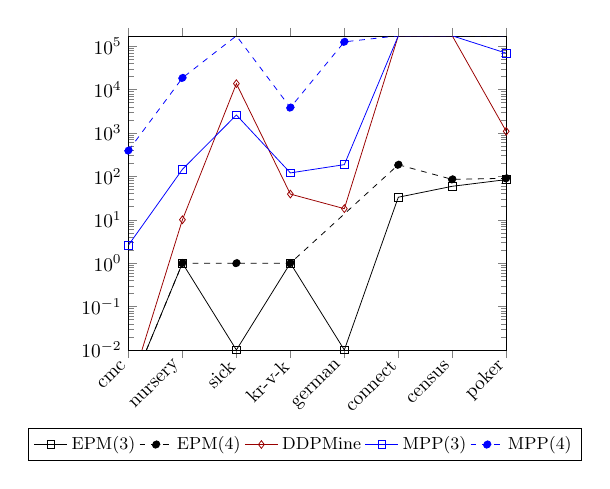
\begin{tikzpicture}[scale = .7]   %
\begin{axis}[
ymin = 0.01, ymax= 170000, legend entries = {EPM(3)\\EPM(4)\\ DDPMine\\ MPP(3)\\MPP(4)\\},ymode=log, %ylabel = Mining Time (Seconds),
legend columns=5, 
legend style={at={(1.2,-0.25)},font=\small}, legend cell align=center,
 draw=none,
 xtick=data,
 xticklabel = {\benchmark{\tick}},
 xtick align=outside,
 ytick align=inside,
 x tick label style={rotate=45,anchor=east},
 title style={font=\Large},
 ylabel near ticks,
 enlarge x limits=false,
xtick distance={400},
 symbolic x coords={cmc,nursery,sick,kr-v-k,german,connect,census,poker},
 ymajorgrids=true,
 grid = none,
 ]
\addplot[
    solid,
    color=black,
    mark=square,
    ]
    coordinates {
    (cmc, 0.001)(nursery, 1)(sick, 0.01)(kr-v-k, 1)(german, 0.01)(connect, 33)(census, 59)(poker, 84)
    };
    \addplot[
    dashed,
    color=black,
    mark=*,
    ]
    coordinates {
    (cmc, 0.001)(nursery, 1)(sick, 1)(kr-v-k, 1)(german,0)(connect, 185)(census, 85)(poker, 90)};
   %     \addplot[
   % dashed,
   % color=black,
   % mark=triangle,
   % ]
   % coordinates {
   % (cmc, 0.001)(nursery, 1)(sick, 3)(kr-v-k, 2)(german,3)(connect, 108)(census, 269)(poker, 238)};
    \addplot[
    solid,
    color=red!60!black,
    mark=diamond,
    ]
    coordinates {
    (cmc, 0.001)(nursery, 10)(sick, 13663)(kr-v-k, 39)(german, 18)(connect, 172800)(census, 172800)(poker, 1090) };
    \addplot[
    color=blue,
    mark=square,
    ]
    coordinates {
    (cmc, 2.6)(nursery, 145)(sick, 2589)(kr-v-k, 120)(german, 186)(connect, 172800)(census, 172800)(poker,68794) };
    \addplot[
    dashed,
    color=blue,
    mark=*,
    ]
    coordinates {
    (cmc, 394)(nursery, 18515)(sick, 172800)(kr-v-k, 3833)(german,125514)(connect, 172800)(census, 172800)(poker, 172800) };

 \end{axis}
\end{tikzpicture}
\end{center}
%}
\caption{Comparison of mining times (seconds).}
\label{fig:all}
\end{figure}
Figure~\ref{fig:all} compares EPM mining time (in seconds) with those of DDPMine and MPP.
The parameter in the parentheses is the pattern size threshold, e.g.\ $\Theta_l=4$ for EPM(4).
The experiments that take more than two days are terminated and are not included.
%TODO As can be seen, increasing $\Theta_l$ does not notably affect the running time of EPM 
%on the datasets with smaller search spaces.
%TODO However, on the datasets with a larger number of frequent items, 
%decreasing $\lambda_1$ affects the processing time more than increasing $\Theta_l$. 
EPM is notably faster in comparison to the other two approaches.
It is notable that the examined datasets are considerably smaller than the coreference data, which includes more than 33 million samples and 200 frequent feature-values.
\begin{table*}[!htb]
    \begin{center}\footnotesize
    \resizebox{\textwidth}{!}{%
    \begin{tabular}{@{}l|l|@{\hskip3pt}rrr@{\hskip3pt}|@{\hskip3pt}rrr@{\hskip3pt}|@{\hskip3pt}rrr@{\hskip3pt}|r@{\hskip3pt}||@{\hskip3pt}rrr@{\hskip3pt}}
     \multicolumn{2}{c}{} & \multicolumn{3}{c}{MUC} &
     \multicolumn{3}{c}{$B^3$} & \multicolumn{3}{c}{CEAF$_e$} & \multicolumn{1}{c}{CoNLL} & \multicolumn{3}{c}{LEA} \\ \hline
     \multicolumn{1}{c}{}& \multicolumn{1}{c}{} &R & P & F$_1$ & R & P & F$_1$ & R & P & F$_1$ &  & R & P & F$_1$\\ \hline
     %\multicolumn{14}{c}{\textbf{CoNLL test set}} \\ \hline
     \hline
     %\multicolumn{14}{c}{deep-coref} \\ \hline
     \parbox[t]{2mm}{\multirow{5}{*}{\rotatebox[origin=c]{90}{ deep-coref}}} 
     & ranking & $70.43$ & $79.57$ & $74.72$ & $58.08$ & $69.26$ & $63.18$ & $54.43$ & $64.17$ & $58.90$ & $65.60$ & $54.55$ & $65.68$ & $59.60$ \\
     & reinforce & $69.84$ & $79.79$ & $74.48$ & $57.41$ & $70.96$ & $63.47$ & $55.63$ & $63.83$ & $59.45$ & $65.80$ & $53.78$ & $67.23$ & $59.76$\\ 
     %ranking-enhanced & $70.08$ & $81.07$ & $75.18$ & $57.90$ & $71.58$ & $64.02$ & $55.07$ & $65.09$ & $59.66$ & $66.20$ & $54.39$ & $68.12$ & $60.49$  \\ 
     &top-pairs & $69.41$ & $79.90$ & $74.29$ & $57.01$ & $70.80$ & $63.16$ & $54.43$ & $63.74$ & $58.72$ & $65.39$ & $53.31$ & $67.09$ & $59.41$  \\ 
	 %& \multicolumn{14}{c}{\textbf{+Linguistic Features}} \\ 
	 %& +linguistic & $69.81$ & $79.46$ & $74.33$ & $57.23$ & $70.35$ & $63.11$ & $54.96$ & $62.74$ & $58.59$ & $65.34$ & $53.48$ & $66.64$ & $59.34$  \\
     &{+EPM} & $71.16$ & $79.35$ & $75.03$ & $59.28$ & $69.70$ & $64.07$ & $56.52$ & $64.02$ & $60.04$ & $66.38$ & $55.63$ & $66.11$ & $60.42$ \\
     &+JIM & $69.89$ & $80.45$ & $74.80$ & $57.08$ & $71.58$ & $63.51$ & $55.36$ & $64.20$ & $59.45$ & $65.93$ & $53.46$ & $67.97$ & $59.85$\\
     \hline
     \parbox[t]{2mm}{\multirow{2}{*}{\rotatebox[origin=c]{90}{ e2e}}} 
     %\multicolumn{14}{c}{e2e-coref} \\ \hline
     & single & $74.02$ & $77.82$ & $75.88$ & $62.58$ & $67.45$ & $64.92$ & $59.16$ & $62.96$ & $61.00$ & $67.27$ & $58.90$ & $63.79$ & $61.25$ \\
     & ensemble & $73.73$ & $80.95$ & $77.17$ & $61.83$ & $72.10$ & $66.57$ & $60.11$ & $65.62$ & $62.74$ & $68.83$ & $58.48$ & $68.81$ & $63.23$\\
     \hline
    \end{tabular}
    }
    \end{center}
    \caption{\footnotesize Comparisons on the CoNLL test set. 
    The F$_1$ gains that are statistically significant: (1) ``+EPM'' compared to ``top-pairs'', ``ranking'' and ``JIM'', (2) ``+EPM'' compared to ``reinforce'' based on MUC, B$^3$ and LEA, (3) ``single'' compared to ``+EPM'' based on MUC and B$^3$, and (4) 
``ensemble'' compared to other systems. Significance is measured based on the approximate randomization test ($p<0.05$) \cite{noreen89}.
    }
    \label{tab:in-domain-evaluations}
\end{table*}

\section{Impact of Informative Feature-values}
\subsection{Experimental Setup}
\label{ch:improvements_baseline}
%For coreference evaluation, we use \emph{MUC} \cite{vilain95}, \emph{B}$^3$ \cite{bagga98b},
%\emph{CEAF}$_e$ \cite{luoxiaoqiang05a}, \emph{LEA} \cite{moosavi16b},
%and the \emph{CoNLL} score, i.e.\ the average F$_1$ value of \emph{MUC}, \emph{B}$^3$, and \emph{CEAF}$_e$.
For determining informative feature-values, 
we extract all features for all mention-pairs\footnote{Each mention is paired with all the preceding mentions.} of the CoNLL training data 
and then apply EPM on this 
data.
In order to prevent learning annotation errors and specific properties of the training data, 
we consider a pattern as frequent if it occurs in coreference relations of at least 
$m$ different coreferring anaphors ($m=20$).
%e.g.\ patterns that only occur in the coreferent relations of a specific anaphor
%that has more than $m$ antecedents will not be included.
Since the majority of mention-pairs are non-coreferent and we are not interested in patterns for non-coreferring relations, 
we also consider the coreference probability of each pattern $p$, i.e.\ $\frac{|\{X_i|p \in X_i \land c(X_i)=coreferent\}|}{|\{X_i|p \in X_i\}|}$, 
in the post-pruning function. 
The coreference probability should be higher than a threshold ($60\%$ in our experiments),
so we only mine patterns that are informative for coreferring mentions.%\footnote{Setting the coreference probability to higher values results in only long and specific patterns.}.

For the coreference resolution experiments, instead of incorporating informative patterns, we incorporate feature-values that are included in the informative patterns mined by EPM.
The reason
is that deep-coref, or any other recent coreference resolver, uses a deep neural network,
which has a fully automated feature generation 
process.
We add these feature-values 
as binary features.

By setting $\Theta_l$ to five,\footnote{We observe that using larger $\Theta_l$ values will result in many over-specified patterns.} EPM results in 
13 pairwise feature-values,
112 POS tags, i.e.\ 53 POS for anaphors and 59 for antecedents,
25 dependency relations,
26 mention types (mention types or fine mention types),
and finally, 14 named entity tags.\footnote{Following the previous studies that show different features are of different importance for various types of mentions, e.g.\ \newcite{denis08} and \newcite{moosavi17a},
we mine a separate set of patterns for each type of anaphor.
These resulting feature-values are the union of informative feature-values for all types of anaphora.}

Based on the observation in Section~\ref{sect:all}, we use the top-pairs model of deep-coref as the baseline to employ additional features, i.e. ``+EPM'' is the top-pairs model in which EPM feature-values are incorporated.
%We measure significant based on the approximate randomization test ($p<0.05$) \cite{noreen89}.

%\footnote{We set the minimum frequency threshold and $\Theta_l$ hyper-parameters 
%only based on the resulting informative feature-values on the training data. }.
%TODO None of the values of the gender, number and animacy features 
%are among the selected feature-values while
%the corresponding compatibility feature-values, i.e.\ ``compatible number=true'', ``compatible gender=true'' and ``compatible animacy=true'', 
%are informative.
%This way we exclude patterns that only occur in the coreferent relations of a specific anaphor
%that has more than 20 antecedents.
%In order to discriminate between coreferent relations of various anaphora, 
%all coreferent relations of a same anaphor are specified with a unique positive label
%that is different from positive labels of other coreferring anaphora.
%All non-coreferring mention pairs are specified with a zero label.
%TODO
%Since we are not interested in patterns for non-coreferring relations, 
%we also consider the coreference probability of each pattern $p$, i.e.\ $\frac{|\{X_i|p \in X_i \land c(X_i)=coreferent\}|}{|\{X_i|p \in X_i\}|}$, 
%in the post-processing step. 
%The coreference probability should be higher than a threshold ($60\%$ in our experiments),
%so we only mine patterns that are informative for coreferring mentions.
%ones\footnote{Setting the coreference probability to higher values results in only long and specific patterns.}.
%The p-value thresholds for both $G^2$ and binomial tests are set to $0.01$.
%For the experiments of this section, we set $\Theta_l$ to 
%five\footnote{Larger values increase the number of informative patterns considerably and result in many specific patterns.}.
%TODO Following the previous studies that show different features are of different importance for various types of mentions \cite{denis08,lassalle13,moosavi17a},
%we mine a separate set of features for each type of anaphor, i.e.\ proper, nominal and pronominal.
%To do so, we separate mention-pairs based on the type of anaphor and mine a separate set of patterns for each type of anaphor.
%TODO Above features are all extracted using the Stanford CoreNLP preprocessing modules\footnote{Available at \url{https://stanfordnlp.github.io/CoreNLP/coref.html}}.
\iffalse

\label{ch:improvements:first_q}
In this section, we show that 
1) the incorporation of all linguistic feature-values does not have a considerable effect on in-domain evaluations,
and 2) the incorporation of informative feature-values significantly improve the performance.

\begin{table}[htbp]
    \begin{center}\footnotesize
    \resizebox{\columnwidth}{!}{%
    \begin{tabular}{@{}l|l|@{\hskip3pt}r@{\hskip3pt}|@{\hskip3pt}r@{\hskip3pt}|@{\hskip3pt}r@{\hskip3pt}|r@{\hskip3pt}||@{\hskip3pt}r@{\hskip3pt}}
     \multicolumn{2}{c}{} & \multicolumn{1}{c}{MUC} &
     \multicolumn{1}{c}{$B^3$} & \multicolumn{1}{c}{CEAF$_e$} & \multicolumn{1}{c}{CoNLL} & \multicolumn{1}{c}{LEA} \\ \hline
     %\multicolumn{1}{c|}{}&R & P & F$_1$ & R & P & F$_1$ & R & P & F$_1$ &  & R & P & F$_1$\\ \hline
     %\multicolumn{6}{c}{\textbf{CoNLL development set}} \\ \hline
     \hline
     %\multicolumn{6}{c}{ranking} \\ \hline
     \parbox[t]{2mm}{\multirow{3}{*}{\rotatebox[origin=c]{90}{\scriptsize  ranking}}} 
     & base  & $74.31$  & $64.23$  & $59.73$ & $66.09$ & $60.47$  \\
	 & +all  & $74.35$  & $63.96$  & $60.19$ & $66.17$ & $60.20$  \\
     & {+EPM}  & $74.91$ & $65.07$ & $60.77$ & $66.92$ & $61.46$  \\
     \hline
     %\multicolumn{6}{c}{top-pairs} \\ \hline
     \parbox[t]{2mm}{\multirow{3}{*}{\rotatebox[origin=c]{90}{\scriptsize  top-pairs}}} 
     & base  & $73.95$ & $63.98$ & $59.52$  & $65.82$ & $60.07$ \\ 
     & +all & $74.32$ & $64.45$ & $60.19$ & $66.32$ & $60.62$ \\
     & +EPM & $74.92$ & $65.03$& $60.88$ & $66.95$ & $61.34$ \\ 
     \hline
    \end{tabular}
    }
    \end{center}
    \caption{Impact of linguistic features on deep-coref models on the CoNLL development set.
    The F$_1$ gains of ``+EPM'' are all statistically significant.}
    \label{tab:top-pair-vs-ranking}
\end{table}
\fi
\iffalse
The impact of linguistic features in deep-coref is shown in Table~\ref{tab:top-pair-vs-ranking}.
The rows ``base'' show the base results of deep-coref's ``ranking'' and ``top-pairs'' models. 
``+all'' represents the results of the mention-ranking models in which the feature set of Section~\ref{sect:base_features} is employed.
For ``+all'', 
the gender, number, animacy and mention type features, which have less than five values, 
are converted to binary features. 
%TODO i.e.\ each feature=value is considered as a binary feature.  
Named entity and POS tags, and dependency relations
are represented as learned embeddings.
As we see, incorporating all the linguistic features bridges the gap between the performance of 
``top-pairs'' and ``ranking''.
However, it does not improve over the ``ranking'' model.
\fi
%Therefore, we use EPM to choose informative values, if any, of the existing features.
%If a feature does not occur in any informative pattern, 
%we exclude it from the set of features.
%\footnote{It takes from two to six hours for mining informative patterns for different types of anaphors.} 
%including 
%TODO deep-coref itself has six pairwise features, i.e.\ three speaker match, exact string match, refined head match and relaxed string match.
%It has a hidden layer of size 1000 on top of the pairwise features.
%The output of the hidden layer is then combined with the output of the hidden layer of word embeddings. 
%Apart from these features, we do not change any other parameter in deep-coref.
%The deep-coref model in which the EPM feature-values are incorporated is referred to as ``+EPM'' in our experiments.
\iffalse
The inclusion of EPM feature-values results in significant improvements.
The F$_1$ gains of ``+EPM'' 
are all statistically significant ($p<0.05$) based on the approximate randomization test \cite{noreen89}.
The results show that linguistic features in which noisy and irrelevant values are discarded
are beneficial for improving the performance of a neural coreference resolver.
%TODO It is worth noting that, as mentioned in Section~\ref{ch:improvement:base_features}, averaged word embeddings are not included in any of the ``+EPM'' experiments. 

For the ``+EPM'' experiments,
the ``top-pairs'' and ``ranking'' models have on-par performance
while ``top-pairs'' uses a simpler objective function and it is used for pretraining the ``ranking'' model.
Henceforth, 
we use the ``top-pairs'' model as the baseline, i.e.\ ``+EPM'' refers to the ``top-pairs'' model with EPM feature-values.
\fi
\subsection{Impact on In-domain Performance}
The performance of the ``+EPM'' model compared to recent state-of-the-art coreference models on the CoNLL test set is presented in Table~\ref{tab:in-domain-evaluations}.
%The ``top-pairs'', ``ranking'', ``reinforce'' rows represent the results of deep-coref's coreference models. 
%The ``+EPM'' row represents the results of deep-coref's top-pairs model in which the EPM feature-values are added.
%The F$_1$ gains of ``+EPM'' compared to all ``top-pairs'', ``ranking'', and ``reinforce'' models are statistically significant.
%The only exception is the difference between ``+EPM'' and ``reinforce'' based on the \emph{CEAF$_e$} metric,
%which is not significant.
The ``single'' and ``ensemble'' rows represent the results of the single and ensemble models of e2e-coref. 

We also compare EPM with the pattern mining approach used by \newcite{uryupina15}, i.e.\ Jaccard Item Mining (JIM).
For a fair comparison, while \newcite{uryupina15} used mined patterns for extracting feature templates, we use them for selecting feature-values.
We run the JIM algorithm on 
the same data and with the same setup as that of EPM.\footnote{
We set the minimum frequency, maximum pattern length and $score^+$ threshold parameters of JIM to 20, 5 and 0.6.}
This results in nine pairwise features, 
260 POS tags, 38 dependency relations, 32 mention types, and 18 named entity tags.
The ``+JIM'' row shows the results of deep-coref top-pairs model 
in which these feature-values are incorporated.
As we see, EPM feature-values result in significantly better performance than those of JIM
while the number of EPM feature-values is considerably less than JIM.
%The difference between the performance of ``+JIM''
%and ``top-pairs'' is statistically significant only based on \emph{MUC}, and \emph{CEAF$_e$} metrics.
%
\begin{table}[!htb]
    \begin{center}\footnotesize
    \begin{tabular}{@{}l|r|r|r|r|r@{\hskip3pt}}
     \multicolumn{1}{c}{} & \multicolumn{1}{c}{MUC} & \multicolumn{1}{c}{$B^3$} & \multicolumn{1}{c}{CEAF$_e$} & \multicolumn{1}{c}{CoNLL} & \multicolumn{1}{c}{LEA} \\ \hline
     %\multicolumn{1}{c|}{}& F$_1$ & F$_1$ & F$_1$ &  & R & P & F$_1$\\ \hline
     \hline
     +EPM  & $74.92$ & $65.03$ & $60.88$ & $66.95$ & $61.34$ \\ \hline
     -pairwise & $74.37$ & $64.55$ & $60.46$ & $66.46$ &$60.71$\\
     -type & $74.71$ & $64.87$ & $61.00$ & $66.86$ & $61.07$\\
     -dep & $74.57$ & $64.79$ & $60.65$ & $66.67$ & $61.01$\\
     -NER & $74.61$ & $65.05$ & $60.93$ & $66.86$ & $61.27$\\
     -POS & $74.74$ & $65.04$ & $60.88$ & $66.89$ & $61.30$\\ \hline
     +pairwise & $74.25$ & $64.33$ & $60.02$ & $66.20$ & $60.57$ \\ 
     \hline
    \end{tabular}
    \end{center}
    \caption{Impact of different EPM feature groups on the CoNLL development set.}
    \label{tab:feature-ablation}
\end{table}

\begin{table*}[!htb]
    \begin{center}\footnotesize
    \resizebox{\textwidth}{!}{%
    \begin{tabular}{@{}l|@{\hskip3pt}l|@{\hskip3pt}rrr@{\hskip3pt}|@{\hskip3pt}rrr@{\hskip3pt}|@{\hskip3pt}rrr@{\hskip3pt}|r@{\hskip3pt}||@{\hskip3pt}rrr@{\hskip3pt}}
     \multicolumn{2}{c}{} & \multicolumn{3}{c}{MUC} &
     \multicolumn{3}{c}{$B^3$} & \multicolumn{3}{c}{CEAF$_e$} & \multicolumn{1}{c}{CoNLL} & \multicolumn{3}{c}{LEA} \\ \hline
     \multicolumn{1}{c}{}& \multicolumn{1}{c}{} &R & P & F$_1$ & R & P & F$_1$ & R & P & F$_1$ &  & R & P & F$_1$\\ \hline
      %\multicolumn{14}{c}{\textbf{WikiCoref}} \\ \hline \hline
         %  \multicolumn{14}{c}{deep-coref} \\ \hline
     \parbox[t]{2mm}{\multirow{5}{*}{\rotatebox[origin=c]{90}{ deep-coref}}} 
      %& conll & $58.59$ & $66.63$ & $62.35$ & $44.40$ & $54.87$ & $49.08$ & $42.47$ & $51.47$ & $46.54$ & $52.65$ & $40.36$ & $50.73$ & $44.95$ \\ 
      &ranking & $57.72$ & $69.57$ & $63.10$ & $41.42$ & $58.30$ & $48.43$ & $42.20$ & $53.50$ & $47.18$ & $52.90$ & $37.57$ & $54.27$ & $44.40$  \\ 
      &reinforce & $62.12$ & $58.98$ & $60.51$ & $46.98$ & $45.79$ & $46.38$ & $44.28$ & $46.35$ & $45.29$ & $50.73$ & $42.28$ & $41.70$ & $41.98$ \\
      &top-pairs & $56.31$ & $71.74$ & $63.09$ & $39.78$ & $61.85$ & $48.42$ & $40.80$ & $52.85$ & $46.05$ & $52.52$ & $35.87$ & $57.58$ & $44.21$\\ 
      &{+EPM} & $58.23$ & $74.05$ & $\boldsymbol{65.20}$ & $43.33$ & $63.90$ & $51.64$ & $43.44$ & $56.33$ & $\boldsymbol{49.05}$ & $\boldsymbol{55.30}$ & $39.70$ & $59.81$ & $\boldsymbol{47.72}$ \\  
      %&+all & $57.29$ & $72.65$ & $64.06$ & $39.68$ & $62.96$ & $48.68$ & $41.61$ & $54.29$ & $47.11$ & $53.29$ & $35.89$ & $58.83$ & $44.58$ \\ \hline
     %      \multicolumn{14}{c}{e2e-coref} \\ \hline
     \parbox[t]{2mm}{\multirow{2}{*}{\rotatebox[origin=c]{90}{ e2e}}} 
      & single & $60.14$ & $64.46$ & $62.22$ & $45.20$ & $51.75$ & $48.25$ & $38.18$ & $43.50$ & $40.67$ & $50.38$ & $40.70$ & $47.56$ & $43.86$ \\
      & ensemble & $59.58$ & $71.60$ & $65.04$ & $44.64$ & $60.91$ & $51.52$ & $40.38$ & $49.17$ & $44.35$ & $53.63$ & $40.73$ & $56.97$ & $47.50$\\ \hline
     & {G\&L} & $66.06$ & $62.93$ & $64.46$ & $57.73$ & $48.58$ & $\boldsymbol{52.76}$ & $46.76$ & $49.54$ & $48.11$ & $55.11$ & - & - & -\\ \hline
    \end{tabular}
    }
    \end{center}
    \caption{Out-of-domain evaluation on the WikiCoref dataset. The highest $F_1$ scores are boldfaced.}
    \label{tab:out-domain-deep-coref}
\end{table*}
\paragraph{Feature Ablation}
Table~\ref{tab:feature-ablation} shows the effect of each group of EPM feature-values, i.e.\ pairwise features, mention types, 
dependency relations, named entity tags and POS tags, on the performance of ``+EPM''.
The performance of ``+EPM'' from which each of the above feature groups is removed, one feature group at a time, 
is represented as ``-pairwise'', ``-types'', ``-dep'', ``-NER'', and ``-POS'', respectively.
%``-pairwise'', ``-types'', ``-dependency'', ``-NER'', and ``-POS'' 
%represent the performance of the ``+EPM'' model in which the corresponding feature group, i.e.\ pairwise, mention type, dependency relations, named entity tags, or POS tags feature-values,
%is removed from EPM feature-values.
The POS and named entity tags have the least 
and the pairwise features have the most significant effect.
Since pairwise features have the most significant effect, 
we also perform an experiment in which only pairwise features are incorporated in the ``top-pairs'' model, i.e.\ ``+pairwise''.
The results of ``-pairwise'' compared to ``+pairwise'' show that pairwise feature-values 
have a significant impact, but only when they are considered in combination with other EPM feature-values.
%

%TODO
%Some feature-values capture competing information,
%e.g.\ POS tags of previous and following words of a mention can implicitly capture whether a mention is a subject or an object, 
%while this information is explicitly captured by dependency relations.
%However,
%we keep them both among the set of feature-values.
%The inclusion of competing features can result in more robust models 
%on test data in which the values of some of these features are noisy or missing \cite{sutton2006reducing}.
%
%
\begin{table}[htbp]
    \begin{center}\footnotesize
    \begin{tabular}{@{}l@{\hskip3pt}|@{\hskip3pt}l@{\hskip3pt}|@{\hskip3pt}r@{\hskip3pt}|@{\hskip3pt}r@{\hskip3pt}||@{\hskip3pt}r@{\hskip3pt}|@{\hskip3pt}r@{}}
         \multicolumn{2}{c}{} & \multicolumn{2}{c}{in-domain} & \multicolumn{2}{c}{out-of-domain} \\ \hline
     %\multicolumn{2}{c|}{} & \multicolumn{1}{c}{CoNLL} & \multicolumn{1}{c||}{LEA} & \multicolumn{1}{c}{CoNLL} & \multicolumn{1}{c}{LEA}  \\ \hline
	 \multicolumn{2}{c}{} & CoNLL & LEA & CoNLL & LEA \\ \hline
          \multicolumn{2}{c}{} & \multicolumn{4}{c}{{pt (Bible)} } \\ \hline
     %top-pairs & $74.48$ & $65.61$ & $74.58$ & $69.81$ & $66.04$ & $51.03$ & $67.73$ & $58.20$\\
	 \multirow{2}{*}{{ deep-coref}}
     &ranking & $75.61$ & $71.00$ & $66.06$ & $57.58$  \\ 
     & +EPM & $76.08$ & $71.13$ & $\boldsymbol{68.14}$ & $\boldsymbol{60.74}$ \\ \hline
     \multirow{2}{*}{{ e2e-coref}} 
     & single& ${77.80}$ & ${73.73}$ & $65.22$ & $58.26$\\ 
	 & ensemble & $\boldsymbol{78.88}$ & $\boldsymbol{74.88}$ & $65.45$ & $59.71$\\
	 \hline 
     \hline
     \multicolumn{2}{c}{} & \multicolumn{4}{c}{{wb (weblog)} } \\ \hline
     %top-pairs & $61.51$ & $48.22$ & $61.58$ & $54.09$ & $58.66$ & $49.65$ & $51.05$ & $50.34$\\
	 \multirow{2}{*}{{ deep-coref}}
     &ranking & $61.46$ & $53.75$ & $57.17$ & $48.74$ \\ 
     &+EPM & $61.97$ & ${53.93}$ & $\boldsymbol{61.52}$ & $\boldsymbol{53.78}$ \\ \hline
     \multirow{2}{*}{{ e2e-coref}}
     &single & ${62.02}$ & $53.09$ & $60.69$ & $52.69$\\ 
	 &ensemble & $\boldsymbol{64.76}$ & $\boldsymbol{57.54}$ & $60.99$ & $52.99$\\
	 
     \hline
    \end{tabular}
    \end{center}
    \caption{In-domain and out-of-domain evaluations for the pt and wb genres of the CoNLL test set.
    The highest scores are boldfaced.
    }
    \label{tab:cross_genre_enhanced_1}
\end{table}
\subsection{Impact on Generalization}
\label{ch:improvements:generalization}
We use the same setup as that of \newcite{moosavi17b} for evaluating generalization 
including (1) training on the CoNLL data and testing on WikiCoref\footnote{WikiCoref only contains 30 documents, which is not enough for training neural coreference resolvers.}
and (2) excluding a genre of the CoNLL data from training and development sets 
and testing on the excluded genre. Similar to \newcite{moosavi17b}, we use the \emph{pt} and \emph{wb} genres for the latter evaluation setup.  
%Following \newcite{moosavi17b}, we use WikiCoref because it has compatible annotation guidelines with CoNLL. 

The results of the first evaluation setup are shown in Table~\ref{tab:out-domain-deep-coref}.
The best performance on WikiCoref is achieved by \newcite{ghaddar16a} (``G\&L'' in Table~\ref{tab:out-domain-deep-coref})
who introduced WikiCoref and design a domain-specific coreference resolver that makes use of 
the Wikipedia markups of a document as well as links to Freebase, which are annotated in WikiCoref.

Incorporating EPM feature-values improves the performance by about three points.
While ``+EPM'' does not use the WikiCoref data during training, and unlike ``G\&L'', it does not employ any domain-specific features,
it achieves on-par performance with that of ``G\&L''.
%We also observe that ``+EPM'' performance is about two point better than ``+linguistic'' (Table~\ref{tab:out_of_domain_linguistics}) on WikiCoref.
This indeed shows the effectiveness of informative feature-values in improving generalization.

%In order to show that the improved generalization is due to incorporating 
%informative feature-values, and not any additional linguistic feature, we also report the performance of ``+all'', 
%i.e.\ ``top-pairs'' in which the feature set of Section~\ref{sect:base_features} is employed.
%As we see, ``+all'' performance is slightly better than ``top-pairs''.
%However, the improvements are not as substantial as those of ``+EPM''. 

%The results of e2e-coref ``single'' vs.\ ``ensemble'' show the effectiveness of ensemble methods for improving generalization.
%By combining ensemble methods, e.g.\ \cite{leekenton17,uryupina-moschitti:2017:CoNLL}, 
%and informative feature-values we can further improve the generalization.
%using an ensemble of ``+EPM'' models is a possible way to further improve the results.

The second set of generalization experiments is reported in Table~\ref{tab:cross_genre_enhanced_1}. 
``in-domain'' columns show the results when the evaluation genres were included in training and development sets 
while the ``out-of-domain'' columns show the results when the evaluation genres were excluded.
As we can see, ``+EPM'' generalizes best, and in out-of-domain evaluations, it considerably outperforms the ensemble model of e2e-coref, which has the best performance on the CoNLL test set. 
%\section{Summary and discussion}\label{s:disc}

In this work we introduced an attack that allows an adversary to violate the 
  guarantees of MPM systems by leveraging users' friends.
We also proposed several mitigations, but our proposals satisfy only two out 
  of three desirable properties: privacy (leak no information), low 
  communication overhead (i.e., clients need not send many messages per round), 
  and low latency (friends get to talk to each other often).
The most pragmatic of our solutions requires bounding the maximum number of 
  friends that a client can have.

Even with our mitigations, compromised friends are a liability and can be
  used to learn sensitive information through other means.
For example, if a user is uncharacteristically slow to respond to a 
  compromised friend's message (a user's response pattern could be constructed over
  many prior interactions), this anomaly in itself leaks information.
We believe that understanding the impact of this type of attack in
  practice is a promising avenue for future work.


\vspace{-3mm}
\section{Conclusion}
\label{sec:conc}
\vspace{-2mm}

%In this paper, we bring a human in the loop to  facilitate the learning process of an image captioning model. 
In this paper, we enable a human teacher to provide feedback to the learning agent in the form of natural language. We focused on the problem of image captioning. 
We proposed a hierarchical phrase-based RNN as our captioning model, which allowed natural integration with human feedback. We crowd-sourced feedback for a snapshot of our model, and showed how to incorporate it in Policy Gradient optimization. We showed  that by exploiting descriptive feedback our model learns to perform better than when given independently written captions. %In the future, we aim to explicitly deal with the annotator 

%There are several exciting avenues for future work. In particular, when dealing with crowd-sourced human reward one needs to take into account annotator noise. We further plan to explore self-criticism, where the agent automatically decides when to seek human advice, possibly in a dialog-like setting. 

\vspace{-3mm}
\section*{Acknowledgment}
\vspace{-3mm}
\begin{small}
We gratefully acknowledge the support from NVIDIA for their donation of the GPUs used for this research. This work was partially  supported by NSERC. We also thank Relu Patrascu for infrastructure support. \end{small}



\section*{Acknowledgments} The authors would like to thank Mark-Christoph M\"uller, Benjamin Heinzerling, Alex Judea, Steffen Eger and the anonymous reviewers for their helpful comments and feedbacks. 
This work has been supported by the Klaus Tschira Foundation, Heidelberg,
Germany and the German Research
Foundation (DFG) as part of the Research Training Group
“Adaptive  Preparation  of  Information  from  Heterogeneous  Sources”  (AIPHES) under  grant  No.
GRK 1994/1. 

\bibliographystyle{acl_natbib_nourl}
\bibliography{mybib}



\end{document}
